% Created 2021-07-14 Wed 15:23
% Intended LaTeX compiler: pdflatex
\documentclass[11pt]{article}
\usepackage[utf8]{inputenc}
\usepackage[T1]{fontenc}
\usepackage{graphicx}
\usepackage{grffile}
\usepackage{longtable}
\usepackage{wrapfig}
\usepackage{rotating}
\usepackage[normalem]{ulem}
\usepackage{amsmath}
\usepackage{textcomp}
\usepackage{amssymb}
\usepackage{capt-of}
\usepackage{hyperref}
\usepackage{kotex}
\hypersetup{colorlinks=true}
\setcounter{secnumdepth}{2}
\author{Hoyoul Park}
\date{\today}
\title{AWS Rails settings}
\hypersetup{
 pdfauthor={Hoyoul Park},
 pdftitle={AWS Rails settings},
 pdfkeywords={org-mode, export, html, theme, style, css, js, bigblow},
 pdfsubject={Org-HTML export made simple.},
 pdfcreator={Emacs 27.2 (Org mode 9.4.4)}, 
 pdflang={English}}
\begin{document}

\maketitle
\tableofcontents

\section{AWS EC2 Server Settings}
\label{sec:org006825f}
\subsection{EC2 생성}
\label{sec:org190e6f6}
\begin{itemize}
\item login한 후에 aws ec2를 만들자.
\begin{enumerate}
\item Launch instance 실행
\end{enumerate}
\end{itemize}
\begin{figure}[htbp]
\centering
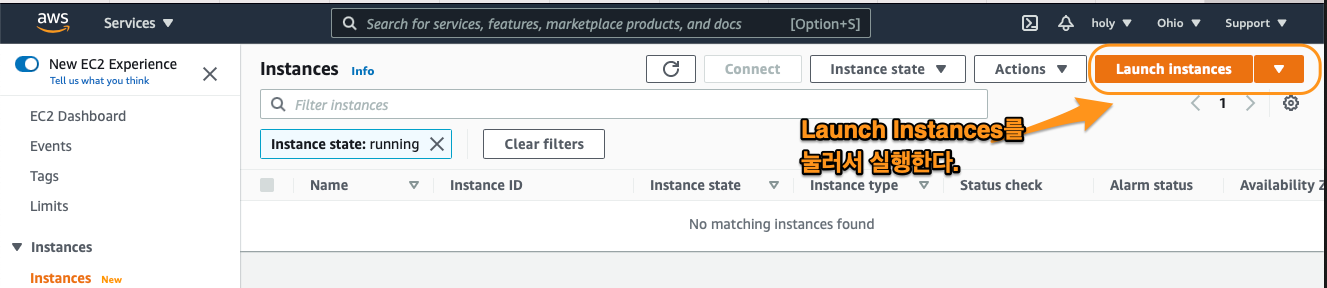
\includegraphics[width=300px]{./img/launchinstance.png}
\caption{\label{fig:orgc3043b0}launch instance}
\end{figure}

\begin{enumerate}
\item ubuntu 20.04를 선택
\end{enumerate}
\begin{figure}[htbp]
\centering
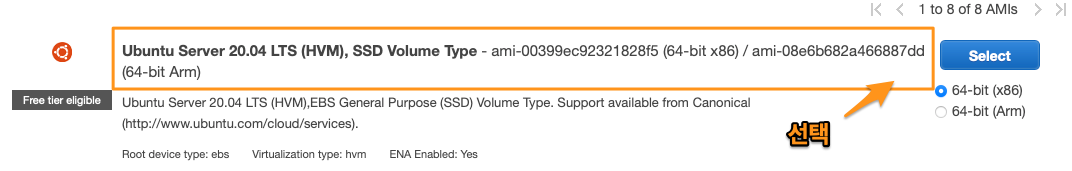
\includegraphics[width=300px]{./img/ubuntu.png}
\caption{\label{fig:org07167e9}ubuntu 20.04 image 선택}
\end{figure}

3)instance를 설정한다.
\begin{figure}[htbp]
\centering
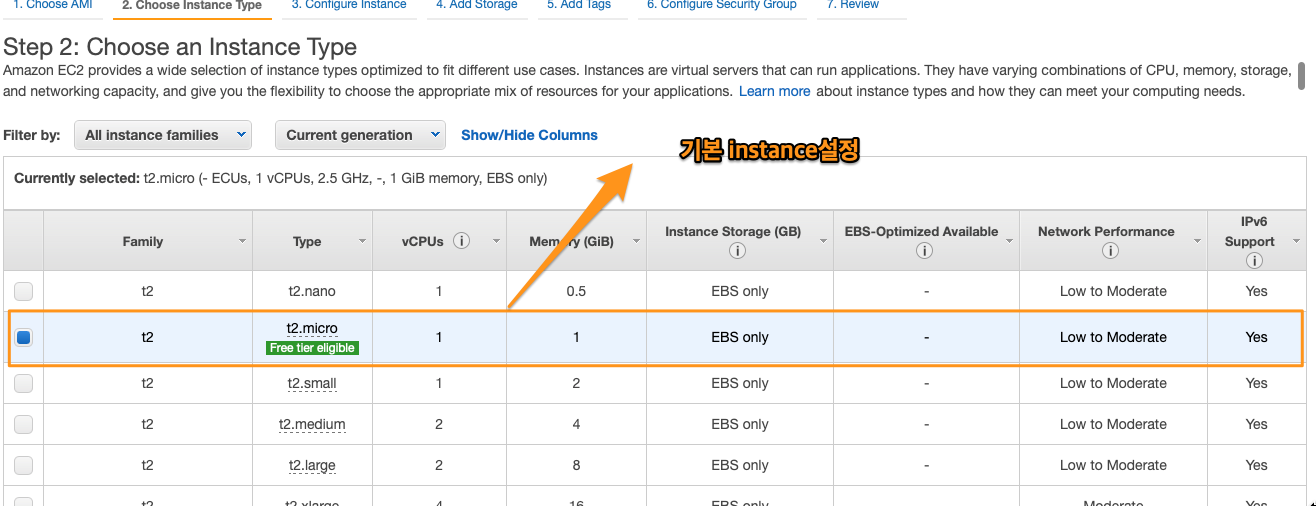
\includegraphics[width=300px]{./img/instance.png}
\caption{\label{fig:org40f3ec7}instance 설정}
\end{figure}

\begin{enumerate}
\item storage(EBS)설정 (돈이 들어간다.)
\end{enumerate}
\begin{figure}[htbp]
\centering
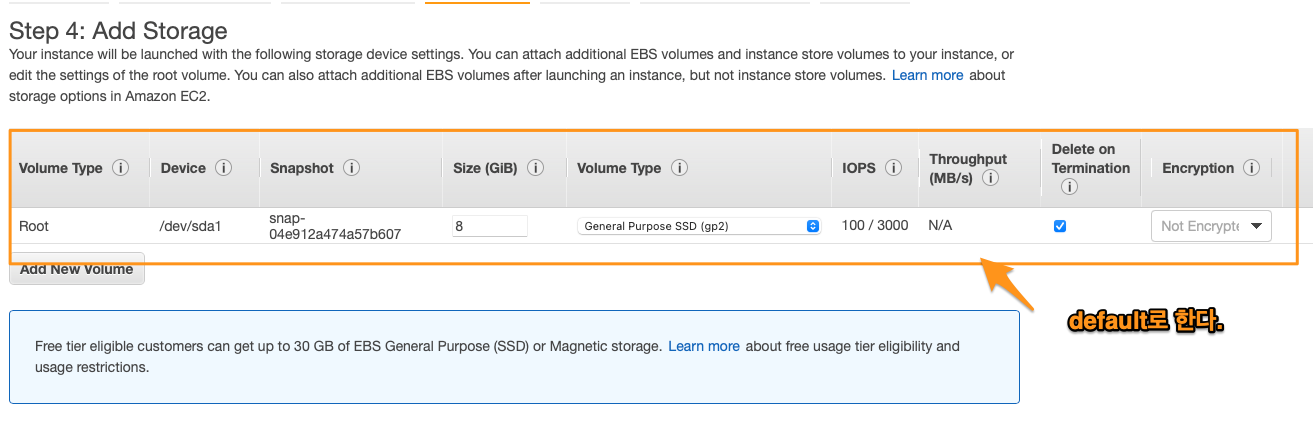
\includegraphics[width=300px]{./img/default.png}
\caption{\label{fig:orgf2edd67}ebs  설정한다.}
\end{figure}

\begin{enumerate}
\item 보안관리자(Security Group)
\end{enumerate}
\begin{figure}[htbp]
\centering
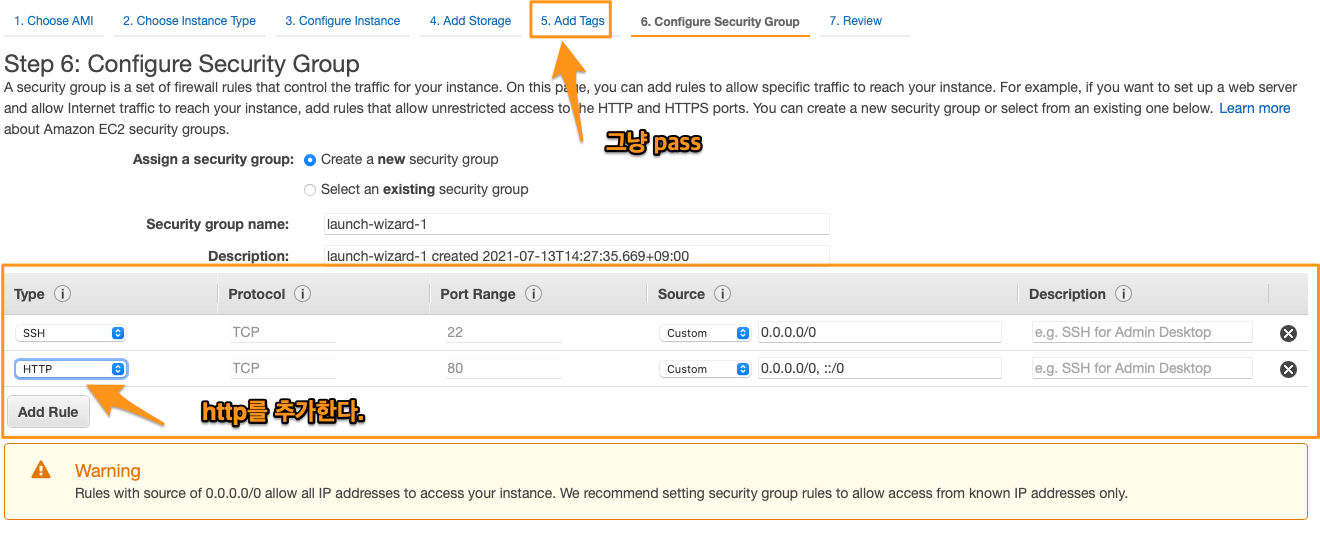
\includegraphics[width=300px]{./img/network.png}
\caption{\label{fig:org14bf488}http추가}
\end{figure}

\begin{enumerate}
\item key 생성
\end{enumerate}
\begin{figure}[htbp]
\centering
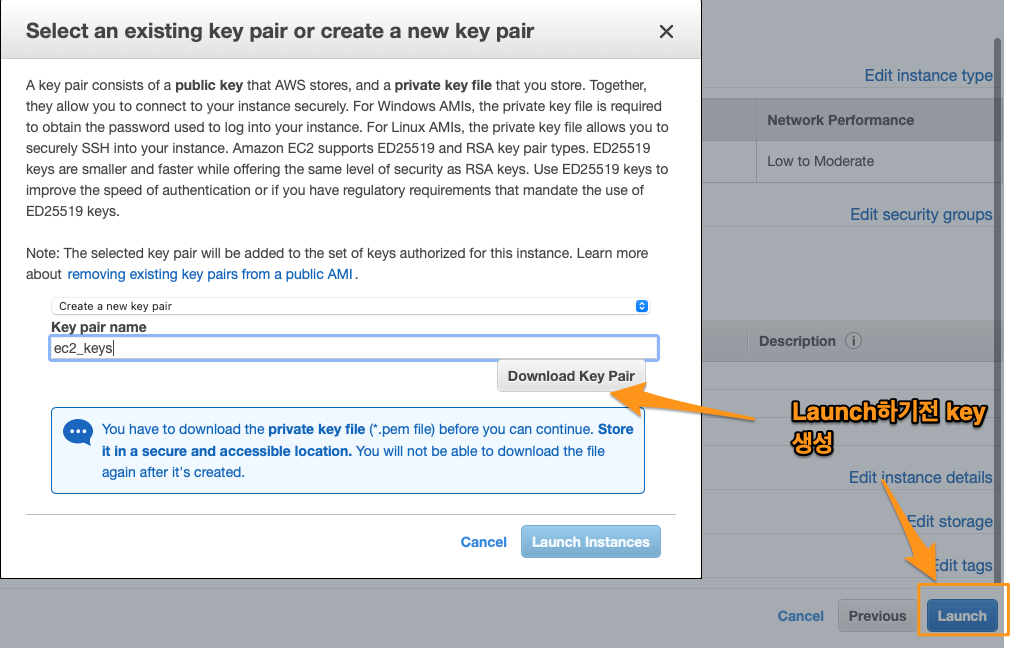
\includegraphics[width=300px]{./img/key.png}
\caption{\label{fig:org6519da2}key}
\end{figure}

\subsection{SSH 접속 settings}
\label{sec:orgc6c0719}
\begin{enumerate}
\item 받은 pem 키를 chmod 0400으로 설정한 후 \textasciitilde{}/.ssh/ 에 넣는다.
\item ec2의 주소를 check한 후 ssh로 접속해보자.
\end{enumerate}
\begin{center}
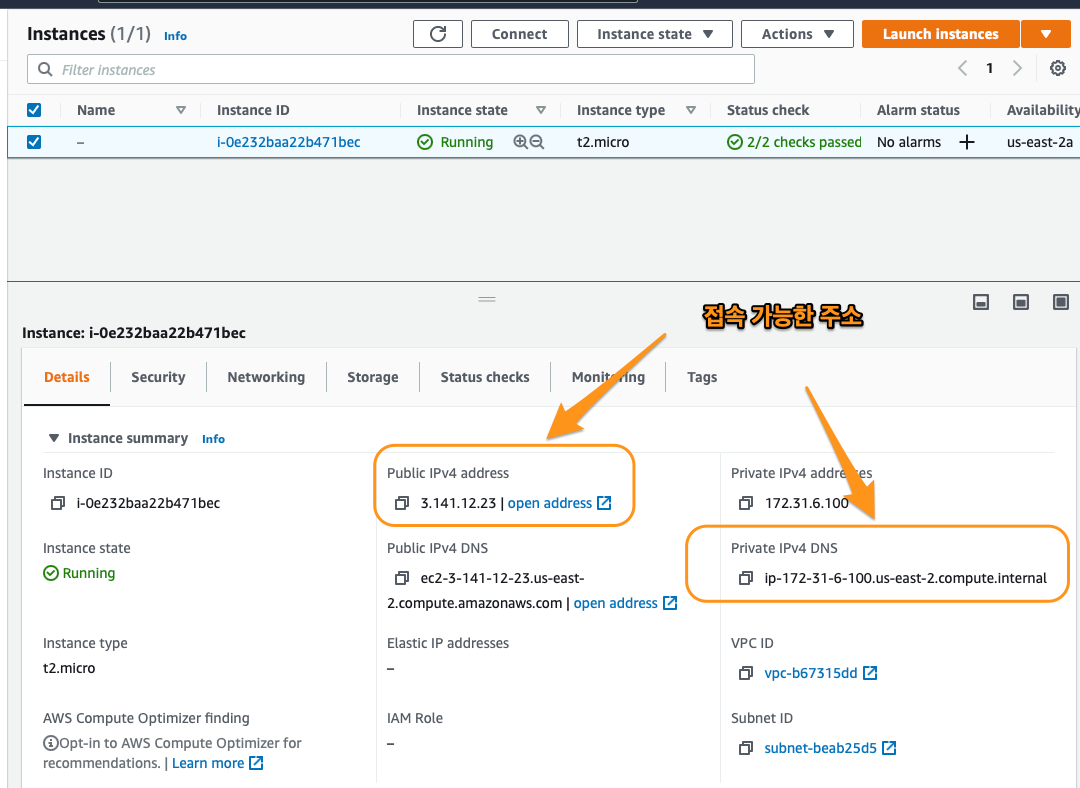
\includegraphics[width=300px]{./img/ssh1.png}
\label{orge8d5af1}
\end{center}

\begin{quote}
ssh -i \textasciitilde{}/.ssh/ec2\textsubscript{keys.pem} ubuntu@주소
\end{quote}
aws에서 설정할 때 얻은 ssh pem 키와 주소를 사용해서 ssh접속을 한다. 주소는 dns주소 혹은 ip주소를 사용해도 된다. 아래에 보면 ubuntu계정으로 접속한 것을 볼 수 있다.
\begin{figure}[htbp]
\centering
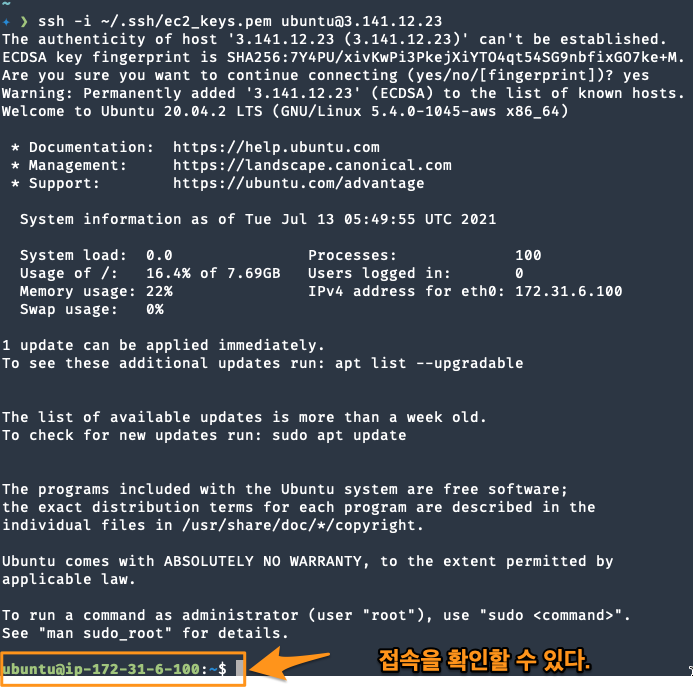
\includegraphics[width=100px]{./img/connection.png}
\caption{\label{fig:org62e498d}connection}
\end{figure}

\subsection{root password설정과 root로 ssh 연결}
\label{sec:orga597807}
\begin{figure}[htbp]
\centering
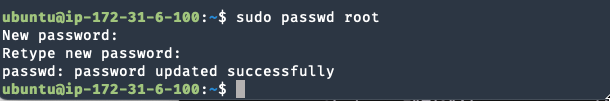
\includegraphics[width=100px]{./img/root_pw.png}
\caption{\label{fig:org8d56246}root password설정}
\end{figure}

\begin{enumerate}
\item ssh 접속을 root로 할 수 있게 설정
\begin{itemize}
\item ubuntu로 접속한다.
\item sudo vi /etc/ssh/sshd\textsubscript{config에서}
\begin{quote}
'\#PermitRootLogin prohibit-password를
PermitRootLogin prohibit-password yes로 바꾼다.
\end{quote}
\end{itemize}
\item su root를 사용해서 root로 switch한다.
\item cd로 home/.ssh으로 이동
\item mv authorized\textsubscript{key} authorized\textsubscript{key}\textsubscript{bak}
\item cp \emph{home/ubuntu}.ssh/authorized\textsubscript{keys} .
현재 ubuntu계정의 ssh키만 aws ec2에 접속할 수 있는 이유는 authorized\textsubscript{key때문이다}. 이 key를 root에 복사해서 root로
접근할 수 있게 하는 것이다.
\item service sshd restart
\end{enumerate}
\begin{figure}[htbp]
\centering
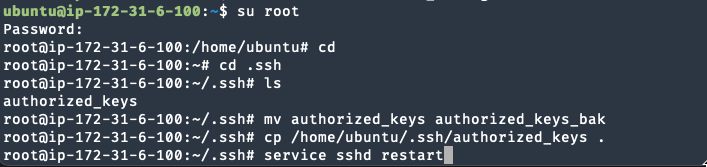
\includegraphics[width=100px]{./img/ssh처리.png}
\caption{\label{fig:orgfd29321}ssh 처리}
\end{figure}
\begin{enumerate}
\item root로 접근이 되는 지 확인해 본다.
\end{enumerate}
\begin{figure}[htbp]
\centering
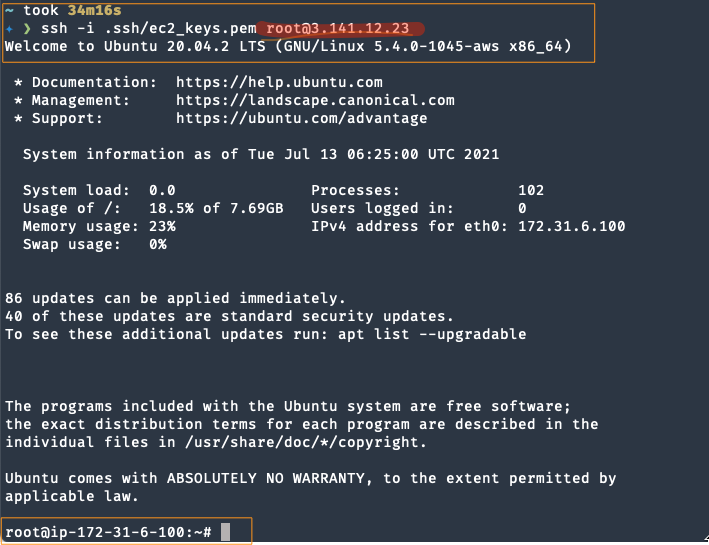
\includegraphics[width=100px]{./img/rootssh.png}
\caption{\label{fig:orgb6bf5a8}root ssh}
\end{figure}

\subsection{deploy를 위한 계정 설정}
\label{sec:orgf4e18b8}
\begin{enumerate}
\item ssh root로 접근
\item deploy계정 생성
\end{enumerate}
\begin{figure}[htbp]
\centering
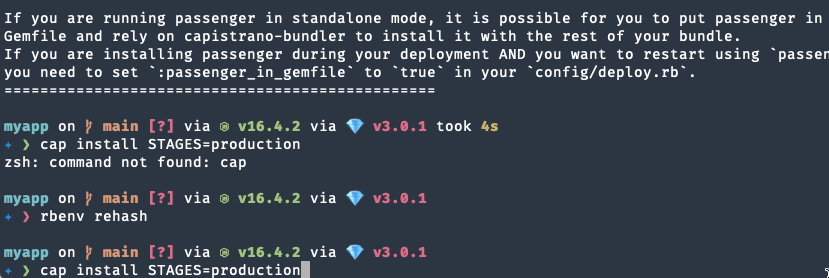
\includegraphics[width=100px]{./img/deploy.png}
\caption{\label{fig:orgecd1460}deploy}
\end{figure}
나머지 설정도 해준다.
\begin{quote}
 
\end{quote}

\begin{enumerate}
\item deploy계정에도 ubuntu, root처럼 ssh 접근이 가능하게 설정한다.
\begin{itemize}
\item sudo mkdir \emph{home/deploy}.ssh
\item sudo cp \emph{home/ubuntu}.ssh/authorized\textsubscript{keys} \emph{home/deploy}.ssh
\item sudo chown -R deploy:deploy \emph{home/deploy}.ssh
\item sudo service sshd restart
\item sudo usermod -aG sudo deploy
\end{itemize}

\item test를 해본다.
\end{enumerate}

\subsection{ruby 설정 (deploy계정으로)}
\label{sec:org8365a94}
\begin{figure}[htbp]
\centering
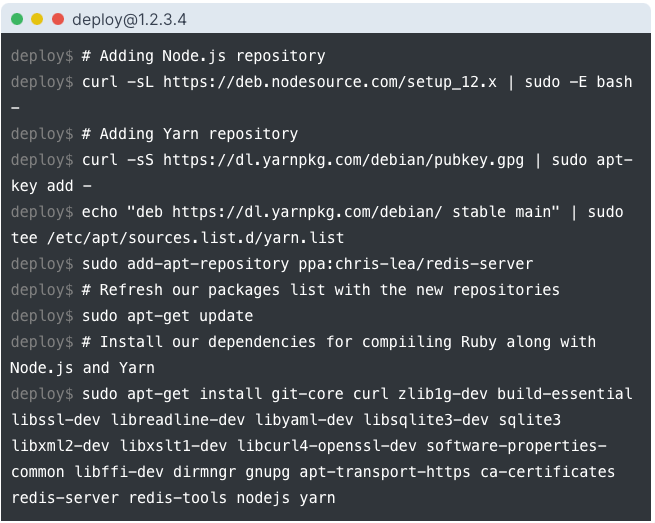
\includegraphics[width=100px]{./img/deploy2.png}
\caption{\label{fig:org6644f5f}deploy2}
\end{figure}

\begin{figure}[htbp]
\centering
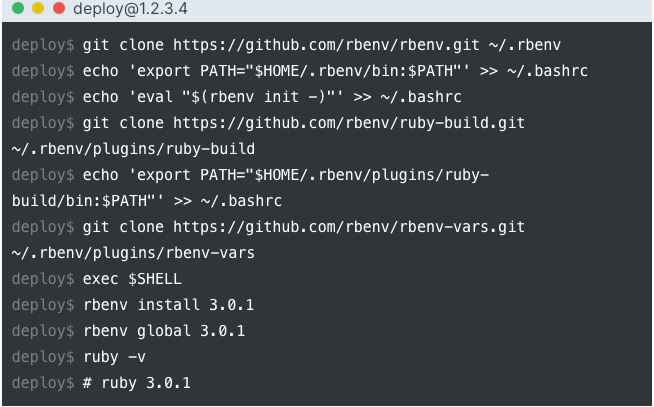
\includegraphics[width=100px]{./img/deploy3.png}
\caption{\label{fig:orge79a7c0}deploy3}
\end{figure}

\subsection{bundler설정}
\label{sec:orgf121310}
\begin{figure}[htbp]
\centering
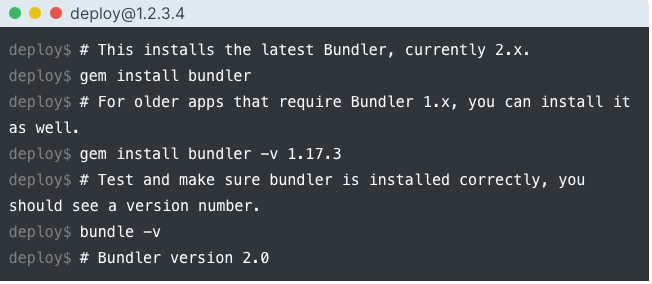
\includegraphics[width=100px]{./img/bundler.png}
\caption{\label{fig:orgcef5eab}bundler}
\end{figure}

\subsection{Nginx \& Passenger 설정}
\label{sec:org2da7c0c}
\begin{figure}[htbp]
\centering
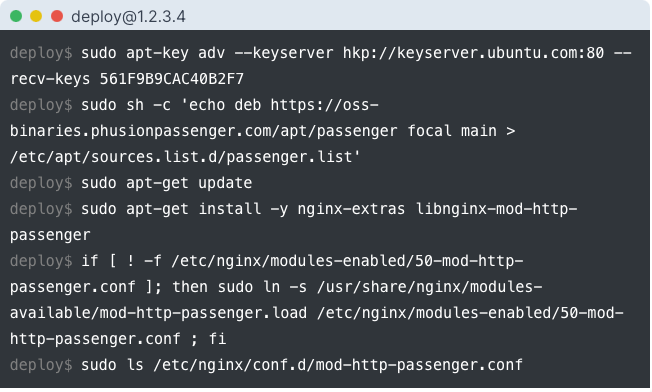
\includegraphics[width=100px]{./img/nginx.png}
\caption{\label{fig:org0726c6e}nginx\&passenger}
\end{figure}

\begin{enumerate}
\item passenger config 파일 수정
\begin{quote}
sudo vi /etc/nginx/conf.d/mod-http-passenger.conf
\end{quote}
아래와 같이 수정한다.
\end{enumerate}
\begin{figure}[htbp]
\centering

\includegraphics[width=100px]{./img/pruby.png}
\caption{\label{fig:org7553984}passenger config}
\end{figure}

\begin{enumerate}
\item nginx를 다시 시작한다.
\begin{quote}
sudo service nginx start
\end{quote}
\item nginx 접속 해 본다.
\end{enumerate}
\begin{figure}[htbp]
\centering
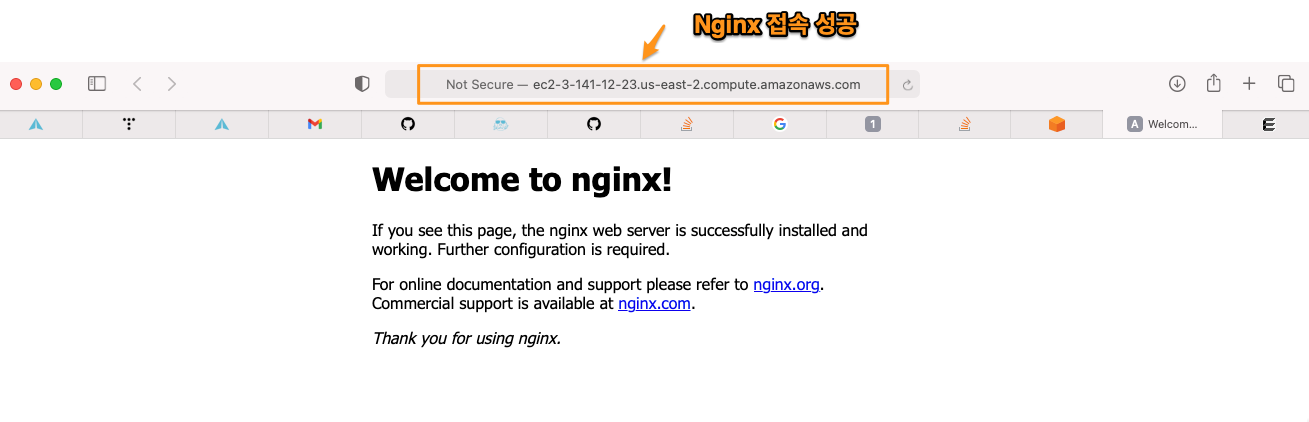
\includegraphics[width=100px]{./img/nginx2.png}
\caption{\label{fig:org766bc85}nginx}
\end{figure}

\begin{enumerate}
\item nginx에 우리의 app을 연결한다.
\end{enumerate}
\begin{figure}[htbp]
\centering
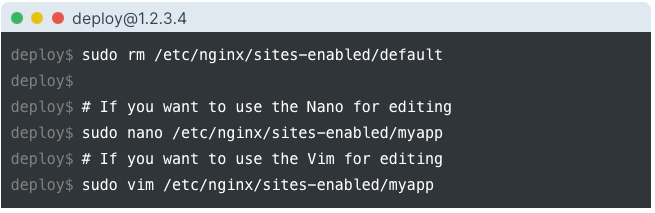
\includegraphics[width=100px]{./img/nginx3.png}
\caption{\label{fig:orgadc9404}nginx associates with my app}
\end{figure}

기존에 연결된 default를 제거하고, 대신 myapp을 설정한다.
그리고 다시 nginx를 다음과 같이 reload한다.
\begin{quote}
sudo service nginx reload
\end{quote}

\begin{itemize}
\item \textbf{Problem}: 예상치 못한 에러 발생
\end{itemize}
\begin{center}
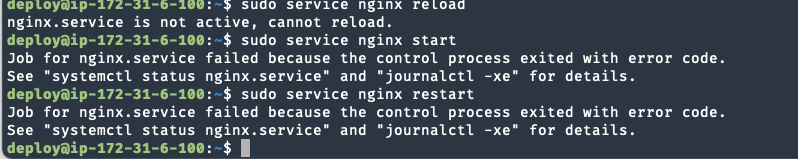
\includegraphics[width=100px]{./img/nginx4.png}
\label{orgf47f87b}
\end{center}
journalctl -xe를 실행해서 에러의 원인이 뭔지 알고 싶었다. 다음과 같은 메시지가 있었다.
\begin{figure}[htbp]
\centering
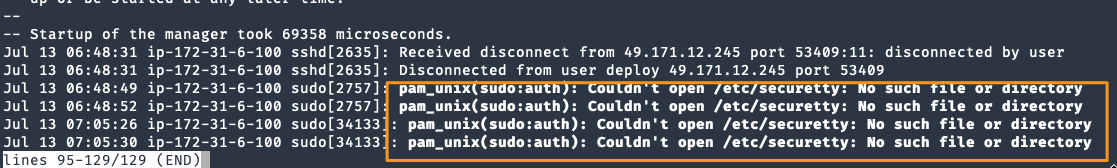
\includegraphics[width=100px]{./img/pam.png}
\caption{\label{fig:org6547a06}pam message}
\end{figure}
더 정확한 확인을 위해서 nginx의 log를 확인해 보자
\begin{figure}[htbp]
\centering
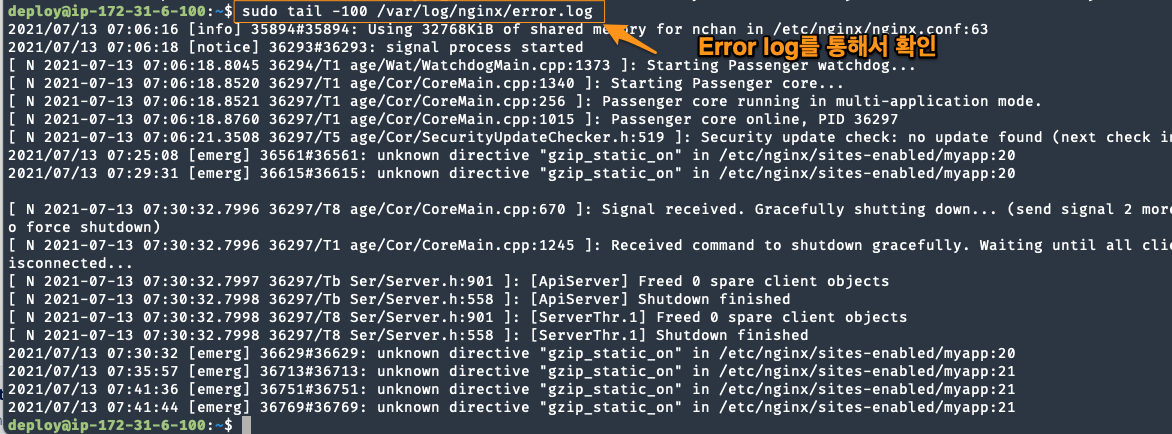
\includegraphics[width=100px]{./img/errorlog.png}
\caption{\label{fig:org3721e5d}error log}
\end{figure}
위에 보면 gzip\textsubscript{static}\textsubscript{on에} 문제가 있어 보인다.

\begin{itemize}
\item \textbf{solution}: gzip\textsubscript{static} on으로 고쳤다.
\end{itemize}
\subsection{Mariadb Database 설치하기}
\label{sec:orgea43c1c}
\begin{enumerate}
\item 우선 system을 업그레이드한다.
\begin{quote}
sudo apt update \&\& sudo apt-get -y upgrade
\end{quote}

\item sudo apt-get install -y mariadb-server
\end{enumerate}
mariadb server를 설치한다.
\begin{enumerate}
\item sudo mysql\textsubscript{secure}\textsubscript{installation}
\end{enumerate}
root pw를 설정한다.
\begin{enumerate}
\item password를 묻는다. 이것은 system password, sudo에 대한..그래서 1234를 입력
\item validation production : y
\item root pw 입력:root1234, 참고로 deploy계정은 pw:user1234
\item anonmous user 삭제:y
\item remote :n
\item testdb delete :y
\item privileges table reload: y
\end{enumerate}
\begin{enumerate}
\item sudo mysql -u root -p
mariadb 설치후에 바로 접속을 시도 해도 접속이 된다.
\end{enumerate}
\begin{figure}[htbp]
\centering
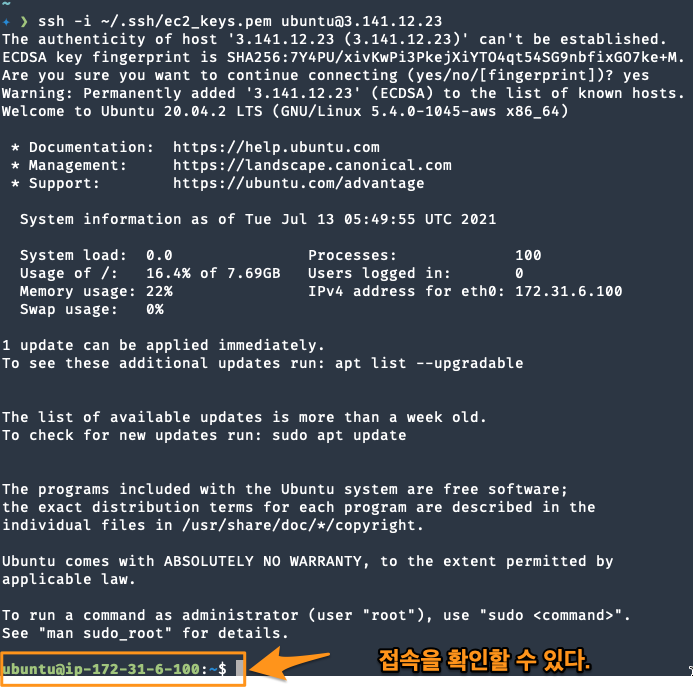
\includegraphics[width=100px]{./img/connection.png}
\caption{\label{fig:org66de6af}mysql connection}
\end{figure}

\begin{enumerate}
\item mariadb에서 database와 user를 만든다.
\end{enumerate}
\begin{figure}[htbp]
\centering
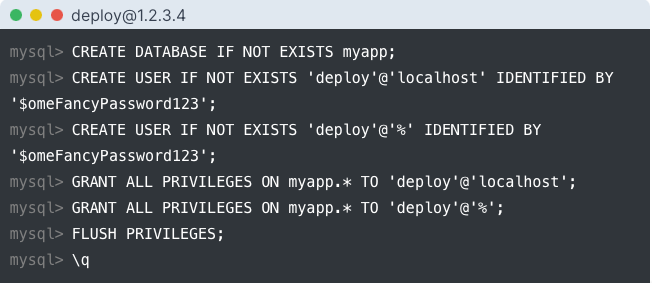
\includegraphics[width=100px]{./img/db_create.png}
\caption{\label{fig:org3b8b270}db \& user}
\end{figure}

\subsection{Capistrano설정}
\label{sec:orgbd97903}
\subsubsection*{Gemfile 설정}
\label{sec:org5cc1cfd}
Local로 다시 들어간다. myapp으로 간다. Gemfiles에 다음을 추가한다.
\begin{quote}
gem 'capistrano', '\textasciitilde{}> 3.11'
gem 'capistrano-rails', '\textasciitilde{}> 1.4'
gem 'capistrano-passenger', '\textasciitilde{}> 0.2.0'
gem 'capistrano-rbenv', '\textasciitilde{}> 2.1', '>= 2.1.4'
\end{quote}
cap명령어를 실행하나 수행되지 않을 때는 rbenv rehash를 하고 다시 실행한다.
\begin{figure}[htbp]
\centering
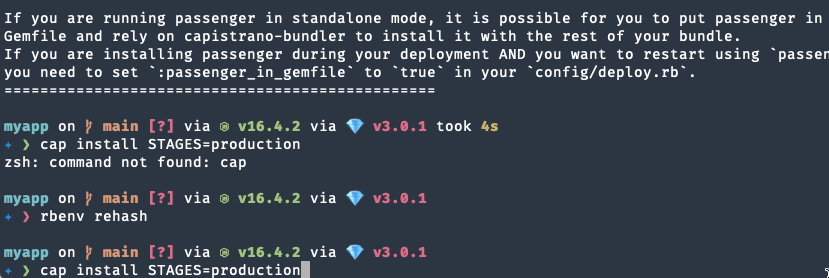
\includegraphics[width=100px]{./img/rehash.png}
\caption{\label{fig:org10b4fcc}rehash}
\end{figure}
\subsubsection*{Capfile 설정}
\label{sec:orgfef2ed3}
이렇게 하면 capfile을 만든다. 그리고 capfile에 다음을 추가한다.
\begin{quote}
require 'capistrano/rails'
require 'capistrano/passenger'
require 'capistrano/rbenv'

set :rbenv\textsubscript{type}, :user
set :rbenv\textsubscript{ruby}, '3.0.1'
\end{quote}
\subsubsection*{config/deploy.rb 설정}
\label{sec:org17f3df7}
\begin{figure}[htbp]
\centering
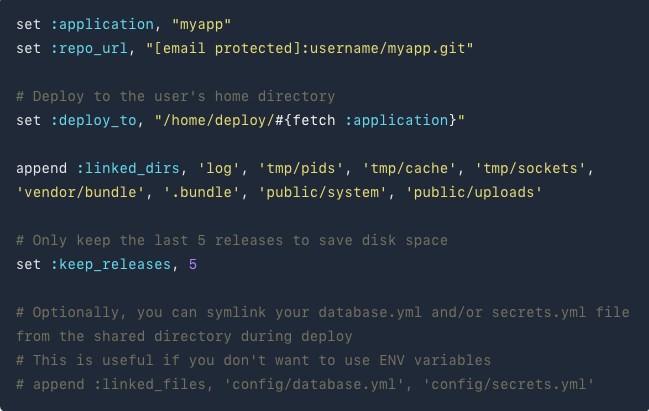
\includegraphics[width=100px]{./img/deploysettings.png}
\caption{\label{fig:org22c106c}deploy settings}
\end{figure}
\end{document}
